\documentclass[11pt]{article}
\usepackage[T1]{fontenc}
\usepackage{lmodern}
\usepackage[margin=1in]{geometry}
\usepackage{amsmath,amssymb,amsthm,mathtools}
\usepackage{microtype}
\usepackage{enumitem}
\usepackage{placeins}
\usepackage{tikz}
\usetikzlibrary{arrows.meta}
\usepackage{xcolor}
\definecolor{linkblue}{RGB}{30,66,115}
\usepackage[colorlinks=true,linkcolor=linkblue,citecolor=linkblue,urlcolor=linkblue]{hyperref}
\hypersetup{pdftitle={Uniform Matrix Hitting Points in Every Positive Characteristic},pdfauthor={OpenAI},pdfsubject={Noncommutative polynomial identity testing}}
\newtheorem{theorem}{Theorem}[section]
\newtheorem{lemma}[theorem]{Lemma}
\newtheorem{proposition}[theorem]{Proposition}
\newtheorem{corollary}[theorem]{Corollary}
\theoremstyle{definition}
\newtheorem{definition}[theorem]{Definition}
\theoremstyle{remark}
\newtheorem{remark}[theorem]{Remark}
\DeclareMathOperator{\Mat}{Mat}
\DeclareMathOperator{\GL}{GL}
\DeclareMathOperator{\ord}{ord}
\newcommand{\F}{\mathbb F}
\newcommand{\J}{\mathcal J}
\newcommand{\eps}{\epsilon}
\newcommand{\articleid}[1]{\begingroup\Urlmuskip=0mu plus 1mu\relax\nolinkurl{#1}\endgroup}
\setlist[enumerate]{itemsep=3pt,topsep=5pt}
\setlength{\emergencystretch}{2em}
\title{Uniform Matrix Hitting Points\\in Every Positive Characteristic}
\author{OpenAI}
\date{October 4, 2026}
\begin{document}
\maketitle
\begin{abstract}
We construct a single matrix substitution that detects every nonzero
size-$s$ division-free noncommutative formula in $n$ variables over every
field of a given positive characteristic. One deterministic machine,
given a promised prime $p$ in binary and $n,s$ in unary, outputs matrices
over $\mathbb F_p$ of dimension $O(n^3s^6)$ in polynomial bit time.
The same tuple works with arbitrary extension-field coefficients,
including in characteristic two. The construction also applies to the
stated acyclic algebraic path programs.
\end{abstract}
\section{Introduction}\label{sec:introduction}

Polynomial identity testing asks whether a polynomial given by arithmetic
operations is zero. In the noncommutative setting, variables are evaluated
on matrices: scalar substitutions would, for example, erase the nonzero
commutator $x_1x_2-x_2x_1$. The question considered here is whether one can
construct a single matrix substitution, using only the characteristic, the
number of variables, and a formula-size bound, that detects every nonzero
formula of that size.
We construct such a substitution over the prime field in every positive
characteristic. Its dimension and the time needed to print all its entries
are polynomially bounded.

\subsection{The result}

For a field $F$, the free associative algebra
$F\langle x_1,\ldots,x_n\rangle$ has as an $F$-basis the finite ordered
words in $x_1,\ldots,x_n$, including the empty word $1$; multiplication
concatenates words. A \emph{noncommutative formula} is a rooted tree whose
leaves are variables or scalars in $F$, and whose internal vertices are
binary addition or ordered multiplication gates. Its \emph{size} is the
number of all vertices, including scalar leaves. Thus there are no inverse
gates and no shared subexpressions. Scalars may be arbitrary elements of $F$.
When evaluating at $d\times d$ matrices, a scalar $a$ is interpreted as $aI_d$.

\begin{theorem}\label{thm:main}
There is a deterministic Turing machine and absolute positive integers $C,k$ with
the following property. Given a prime $p$ in binary and positive integers
$n,s$ in unary, the machine outputs a positive integer $d=O(n^3s^6)$ and
a tuple
\[
 (T_1,\ldots,T_n)\in\Mat_d(\F_p)^n.
\]
For every field $F$ of characteristic $p$ and every nonzero
$f\in F\langle x_1,\ldots,x_n\rangle$ computed by a formula of size at
most $s$, the same tuple, viewed over $F$, satisfies
\[
 f(T_1,\ldots,T_n)\ne0.
\]
Writing $L=\lceil\log_2p\rceil$, the total running time and output length
are at most $C(n+s+L+1)^k$. All matrix entries are output densely as ordinary
binary residues in $\{0,\ldots,p-1\}$, with dimensions and separators included.
Primality of $p$ is promised.
\end{theorem}

The generator receives no formula or coefficients. In particular, its
guarantee is uniform over arbitrary extensions of $\F_p$, and applies to
$p=2$ without any relation between the characteristic and the formula size.
The required conclusion is matrix nonvanishing. The time to evaluate a
formula over an unspecified coefficient field is separate from the bit
complexity of constructing the tuple.

The proof also applies to an \emph{acyclic algebraic path program}: a finite
directed acyclic graph with a designated source and sink, edges labelled by
scalars or variables, and value equal to the sum of ordered label products
over source--sink paths. Replacing the formula-size parameter by the number
of vertices gives the same polynomial construction; see
Corollary~\ref{cor:path-programs}. This extension follows from the coefficient
representation used in the proof.

\subsection{Context and the characteristic obstruction}

Noncommutative identity testing has distinct tests that use the internal
representation and tests that only evaluate the polynomial. Nisan
characterized homogeneous noncommutative branching-program complexity by
ranks of coefficient matrices~\cite[Theorem~1]{Nisan1991}. Raz and Shpilka gave
a deterministic polynomial-time identity test for noncommutative formulas
and algebraic branching programs when their descriptions are
available~\cite{RS2005}. Matrix evaluation also underlies randomized
black-box tests; Bogdanov and Wee gave such a test for circuits with a
supplied degree bound, using polynomial identities of matrix
algebras~\cite[Theorem~4.2]{BW2005}.

For deterministic black-box testing, Forbes and Shpilka constructed
quasipolynomial-size matrix hitting sets for noncommutative algebraic
branching programs, under a field-cardinality hypothesis
\cite[Corollary~4.7]{FS2013}. A block-diagonal sum can combine a finite
hitting set into one tuple, but its dimension grows with the size of that
set. Lakhani and Mukhopadhyay constructed one integer matrix tuple for
sparsity-bounded polynomials over characteristic-zero fields
\cite[Theorem~2.1 and Remark~2.6]{LM2026}; their finite-field formulation
also distinguishes a succinct extension-field description from its explicit
coordinate cost. Sparsity is a different parameter: a formula of small size
can have exponentially many words. These results provide relevant
benchmarks, while the construction here is polynomial in formula size
and in the binary length of the characteristic.

The characteristic-zero companion~\cite[Theorem~1.1]{OAInc} constructs one
rational matrix tuple for formulas, with dimension at most $2ns^2$ and
polynomial bit complexity. Its proof encodes words by iterated integrals,
puts the encoding of a formula into a finite differential system, and
applies an order-of-vanishing bound before truncating. The representation
by an acyclic path program is independent of the characteristic. The
analytic-looking part of the construction is not: formal integration
divides by positive integers, ordinary differentiation annihilates
$p$th powers in characteristic $p$, and distinct integer pole locations
may coincide. Nor does reduction of a rational hitting tuple automatically
preserve its guarantee at every prime.

We retain the word-series and matrix-system organization, replacing the
differential operator by an infinite-order multiplicative shift. The
resulting order bound and the final descent to prime-field matrices are
proved directly in the given characteristic. The dimension bound is larger
than in the companion, but remains polynomial without any lower bound on $p$.

\subsection{Proof strategy}

Fix an arbitrary coefficient field $F$ and introduce an indeterminate $t$
over it. Over $K=F(t)$, let $\sigma$ act on formal series in $z$ by
$\sigma(g)(z)=g(tz)$. For each letter $i$, define the operator $\J_i$ by
requiring $\J_i(g)$ to have zero constant term and
\[
 (\sigma-1)\J_i(g)=\frac{z}{1-(1+t)^i z}\,g.
\]
On the coefficient of $z^r$ for $r\ge1$, this divides by $t^r-1$, which is nonzero
in every characteristic. Iteration defines a series $h_w$ for each word
$w$, starting from $h_\eps=1$ for the empty word $\eps$.
Section~\ref{sec:words} proves that these series are linearly independent.
A minimal-relation argument reduces the claim to a pole obstruction:
a difference $\sigma(R)-R$, with $R\in K(z)$, cannot have just one pole
in an infinite shift orbit,
whereas the poles $(1+t)^{-i}$ lie in disjoint such orbits.
Thus a nonzero polynomial $f=\sum_w f_wx_w$ gives a
nonzero series $h_f=\sum_w f_wh_w$.

Formula size bounds how late the first nonzero coefficient of $h_f$ can
appear. Section~\ref{sec:systems} finds a row $u$, a column $v$, and
strictly upper triangular $m\times m$ matrices $B_1,\ldots,B_n$ over $F$,
with $m\le2s$, such that $f_w=uB_wv$; here
$B_{i_1\cdots i_\ell}=B_{i_1}\cdots B_{i_\ell}$ and $B_\eps=I_m$.
The finite sum $H=\sum_w B_wh_w$ satisfies $H(0)=I$ and
$\sigma(H)=(P/Q)H$, with $z$-degrees at most $n$ and $Q(0)=1$.
Section~\ref{sec:order} proves the reusable bound
\[
 uHv\ne0\quad\Longrightarrow\quad
 \ord_z(uHv)\le n\binom m2.
\]
The proof adapts the determinant method for differential systems: a basis
of series with distinct leading orders $c_i$ has a shifted determinant
whose leading coefficient is a Vandermonde determinant on $t^{c_i}$.
These elements remain distinct in small characteristic. Rational degree
bounds then control the orders of the relevant minors.

Truncating in $z$ now gives matrices over $\F_p(t)$ that detect all the
required formulas. Section~\ref{sec:construction} removes $t$ without
choosing a large finite extension. Strict triangularity supplies one
denominator clearing every evaluated word, together with a polynomial
bound on the remaining $t$-degree. Reduction modulo a sufficiently large
power $t^E$ preserves nonvanishing. Finally, representing multiplication
on $\F_p[t]/(t^E)$ by matrices over $\F_p$ gives the output tuple.
The shift order bound is useful independently of the formula application;
the last step is a general way to retain bounded-degree rational data in
ordinary matrices over the base field.

\section{Independent word series from a multiplicative shift}\label{sec:words}

We first encode free polynomials by formal power series without losing any
nonzero polynomial. No size bound is needed in this section. Fix a field $F$,
let $t$ be an indeterminate over $F$, and put $K=F(t)$. For a second formal
variable $z$, define
\[
 \sigma:K((z))\longrightarrow K((z)),\qquad
 \sigma(g)(z)=g(tz).
\]
This automorphism fixes $K$ and preserves both $K[[z]]$ and $K(z)$, where
rational functions are embedded by Laurent expansion at $z=0$.
Since $t^r\ne1$ for every nonzero integer $r$, coefficient comparison gives
\begin{equation}\label{eq:fixed-field}
 K((z))^\sigma=K.
\end{equation}
In particular, this remains true when the characteristic divides $r$.

For $1\le i\le n$, set
\begin{equation}\label{eq:letters}
 a_i=(1+t)^i,\qquad b_i(z)=\frac{z}{1-a_i z}.
\end{equation}
Given $g\in K[[z]]$, define $\J_i(g)$ to be the unique series
$h\in zK[[z]]$ satisfying
\begin{equation}\label{eq:shift-antiderivative}
 (\sigma-1)h=b_i g.
\end{equation}
Indeed, the right side has zero constant coefficient, and the coefficient
of $z^r$ in $h$, for $r\ge1$, is obtained by dividing the corresponding coefficient of
$b_i g$ by $t^r-1$. Thus $\J_i$ is $K$-linear and
\begin{equation}\label{eq:order-raising}
 \J_i\bigl(z^jK[[z]]\bigr)\subseteq z^{j+1}K[[z]]\qquad(j\ge0).
\end{equation}
The role of the transcendental parameter is already visible: all these
divisions are valid in every characteristic.

Let $\{1,\ldots,n\}^*$ denote the set of finite words, including the empty
word $\eps$. For $w=i_1\cdots i_\ell$, write
$x_w=x_{i_1}\cdots x_{i_\ell}$, with $x_\eps=1$. Define
\begin{equation}\label{eq:word-series}
 h_\eps=1,\qquad h_{iw}=\J_i(h_w),
\end{equation}
where $iw$ means that $i$ is prefixed to $w$.
Our objective is to prove that these series are linearly independent, even
with rational-function coefficients. The relevant obstruction is that a
rational difference cannot have an isolated pole in an infinite shift orbit.
Such pole-orbit obstructions are central to rational $q$-summation;
see Chen and Singer~\cite[Section~2.3]{ChenSinger2012} for a systematic
residue criterion in characteristic zero. The elementary form needed here
has the following proof in arbitrary characteristic.

\begin{lemma}[A rational difference obstruction]\label{lem:poles}
With $K$, $\sigma$, and $b_1,\ldots,b_n$ as above, suppose
\[
 \sum_{i=1}^n c_i b_i=\sigma(R)-R,
 \qquad c_i\in K,\quad R\in K(z).
\]
Then $c_1=\cdots=c_n=0$.
\end{lemma}

\begin{proof}
The unique finite pole of $b_i$ is $\alpha_i=(1+t)^{-i}$, a nonzero
element of $K$. The orbits
\[
 \mathcal O_i=\{t^j\alpha_i:j\in\mathbb Z\}
\]
are infinite and pairwise disjoint. To check the latter assertion, an orbit
intersection would give $(1+t)^{i-i'}=t^a$ for an integer $a$.
The order at $t=0$ forces $a=0$, and the order at $t=-1$ then forces
$i=i'$. Orders of rational functions are integers; this reasoning is
unchanged when the characteristic divides $i-i'$.

Suppose $c_i\ne0$. The left side has exactly one pole on $\mathcal O_i$.
The rational function $R$ has only finitely many poles there.
If it has none, neither does $\sigma(R)-R$. Otherwise let $j_-$ and $j_+$
be the smallest and largest indices of its poles in this orbit.
Substitution $z\mapsto tz$ moves each pole from index $j$ to index $j-1$.
At index $j_--1$, only $\sigma(R)$ has a pole; at index $j_+$, only $-R$
has one. These are two distinct poles of $\sigma(R)-R$, a contradiction.
The argument does not depend on the pole orders or on cancellation at
interior indices; Figure~\ref{fig:poles} illustrates precisely this point.
\end{proof}

\begin{figure}[tb]
\centering
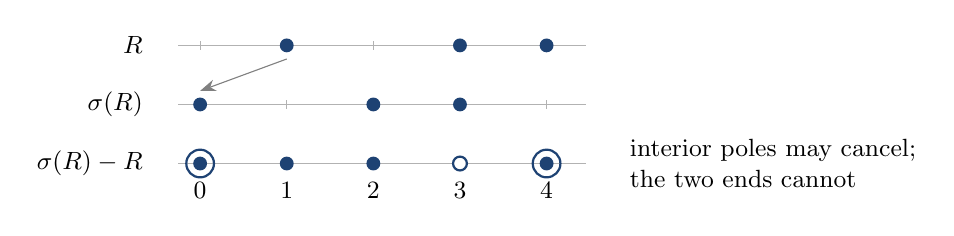
\begin{tikzpicture}[x=1.1cm,y=0.75cm,font=\small]
 \foreach \y/\lab in {2/{$R$},1/{$\sigma(R)$},0/{$\sigma(R)-R$}} {
  \node[anchor=east] at (-0.55,\y) {\lab};
  \draw[gray!60] (-0.25,\y)--(4.45,\y);
  \foreach \j in {0,...,4} \draw[gray!60] (\j,\y-0.07)--(\j,\y+0.07);
 }
 \foreach \j in {1,3,4} \fill[linkblue] (\j,2) circle (2.5pt);
 \foreach \j in {0,2,3} \fill[linkblue] (\j,1) circle (2.5pt);
 \foreach \j in {0,1,2,4} \fill[linkblue] (\j,0) circle (2.5pt);
 \draw[linkblue,fill=white,thick] (3,0) circle (2.5pt);
 \draw[linkblue,thick] (0,0) circle (5pt);
 \draw[linkblue,thick] (4,0) circle (5pt);
 \draw[-{Stealth[length=2mm]},gray] (1,1.77)--(0,1.23);
 \foreach \j in {0,...,4} \node[below] at (\j,-0.15) {$\j$};
 \node[anchor=west,align=left] at (4.85,0) {interior poles may cancel;\\the two ends cannot};
\end{tikzpicture}
\caption{Pole indices in one orbit $\{t^j\alpha:j\in\mathbb Z\}$,
illustrated with pole set $\{1,3,4\}$ for $R$.
The shift lowers indices by one. The open point allows cancellation at
an overlapping pole, while the circled endpoint poles always survive.
The proof uses the same endpoint argument for every finite nonempty pole set.}
\label{fig:poles}
\end{figure}
\FloatBarrier

The proof below is a shift analogue of the minimal-relation argument for
differential word series in Deneufch\^atel, Duchamp, Hoang Ngoc Minh, and
Solomon~\cite[Theorem~1]{Deneufchatel2011}. We include the argument:
$\sigma-1$ is not a derivation, and the field here may have positive
characteristic.

\begin{proposition}[Word-series independence]\label{thm:words}
For every field $F$ and every positive integer $n$, the series
$(h_w)_{w\in\{1,\ldots,n\}^*}$ in~\eqref{eq:word-series} are linearly
independent over $F(t)(z)$.
\end{proposition}

\begin{proof}
Suppose there is a nontrivial finite relation
\begin{equation}\label{eq:minimal-relation}
 \sum_w R_w h_w=0,\qquad R_w\in K(z).
\end{equation}
Choose one with smallest maximum occurring word length $\ell$, then with
fewest nonzero coefficients at length $\ell$. Since $h_\eps=1$, we have
$\ell\ge1$. Divide by one nonzero length-$\ell$ coefficient to make it $1$.

Apply $\sigma$ to~\eqref{eq:minimal-relation} and subtract the original
relation. By~\eqref{eq:shift-antiderivative}, the coefficient of $h_w$ in
the resulting relation is
\begin{equation}\label{eq:new-relation}
 \widetilde R_w=\sigma(R_w)-R_w+
          \sum_{i=1}^n b_i\sigma(R_{iw}),
\end{equation}
where missing coefficients are zero. This relation has no words longer
than $\ell$, introduces no new length-$\ell$ coefficient, and removes
the normalized coefficient. If any $\widetilde R_w$ were nonzero, one
of the two minimality conditions would fail. Therefore all of them vanish.

For $|w|=\ell$, Equation~\eqref{eq:new-relation} gives
$\sigma(R_w)=R_w$, so~\eqref{eq:fixed-field} implies $R_w\in K$.
For each $|w|=\ell-1$, it then gives
\[
 \sum_{i=1}^n b_i R_{iw}=\sigma(-R_w)-(-R_w).
\]
Lemma~\ref{lem:poles} forces every $R_{iw}$ to vanish. Every word of
length $\ell$ occurs in exactly one such family, contradicting the
choice of the original relation.
\end{proof}

For a free polynomial $f=\sum_w f_w x_w$ over $F$, put
\begin{equation}\label{eq:hf}
 h_f=\sum_w f_w h_w=f(\J_1,\ldots,\J_n)1.
\end{equation}
The rightmost operator acts first, so the second equality follows from
the prefix convention in~\eqref{eq:word-series}. Proposition~\ref{thm:words}
shows that $f\ne0$ implies $h_f\ne0$. To turn this encoding into finite
matrices, we must now bound how far into $h_f$ its first nonzero coefficient
can occur. Formula size supplies that bound through a finite matrix system.

\section{From formulas to finite shift systems}
\label{sec:systems}

The word series of Section~\ref{sec:words} send every nonzero polynomial
$f=\sum_w f_w x_w$ to a nonzero series $h_f=\sum_w f_w h_w$.
To bound the order of this series in terms of formula size, we first represent
the word coefficients $f_w$ by matrices of bounded dimension.  We use the standard passage
from formulas to path programs~\cite[Section~2.1, Lemma~2, Step~1]{RS2005}
and the resulting coefficient representation~\cite[Lemma~3.1]{OAInc}.
We give the construction over an arbitrary field, keeping track of scalar
edges and the order of multiplication.

An \emph{acyclic scalar/variable-labelled path program} over a field $F$ is a
finite directed acyclic graph, with parallel edges allowed, whose edges are
labelled by scalars in $F$ or by variables $x_1,\ldots,x_n$.  It has designated
source and sink vertices; these vertices may coincide and need not be first
and last in a topological ordering.  The value of a directed path is the
product of its edge labels in traversal order.  The value of the program is
the sum of these products over all paths from the designated source to the
designated sink.  When the two vertices coincide, the empty path contributes
$1$.  Acyclicity makes this a finite sum in
$F\langle x_1,\ldots,x_n\rangle$.

\begin{lemma}[Coefficient representation of a path program]
\label{lem:acyclic-representation}
Let $F$ be a field, and let a path program with $m\geq 1$ vertices have value
$f=\sum_w f_w x_w$.  There are a row $u\in F^{1\times m}$, a column
$v\in F^{m\times 1}$, and strictly upper triangular matrices
$B_1,\ldots,B_n\in\Mat_m(F)$ such that
\begin{equation}
\label{eq:coefficient-representation}
 f_w=uB_wv,
 \qquad
 B_{i_1\cdots i_\ell}=B_{i_1}\cdots B_{i_\ell},
 \qquad B_\eps=I_m.
\end{equation}
In particular, $B_w=0$ whenever $|w|\geq m$.
\end{lemma}

\begin{proof}
Number the vertices in a topological order, so every edge goes from a smaller
index to a larger one.  Matrix rows index starting vertices and columns index
ending vertices.  Let $(E_0)_{ab}$ be the sum of the scalar labels on edges
from $a$ to $b$.  Let $(X_i)_{ab}$ be the sum of one copy of $1_F$ for each
edge from $a$ to $b$ labelled $x_i$.  All these matrices are strictly upper
triangular.  Consequently
\[
 S=I_m+E_0+\cdots+E_0^{m-1}
\]
has as its $(a,b)$ entry the sum of the values of all scalar-only paths from
$a$ to $b$, including the empty path when $a=b$.

Write $\mathrm{src}$ and $\mathrm{snk}$ for the designated vertices, and let
$e_a$ denote the $a$th coordinate column.  A path whose sequence of variable
labels is $i_1\cdots i_\ell$ decomposes uniquely into scalar-only paths
separated by these variable edges.  Since scalar labels are central, summing
over these decompositions gives
\begin{equation}
\label{eq:scalar-path-elimination}
 f_{i_1\cdots i_\ell}
 =e_{\mathrm{src}}^{\mathsf T}
   S X_{i_1}S\cdots X_{i_\ell}S e_{\mathrm{snk}}.
\end{equation}
For the empty word the right-hand side is
$e_{\mathrm{src}}^{\mathsf T}S e_{\mathrm{snk}}$.
Taking
\[
 u=e_{\mathrm{src}}^{\mathsf T}S,
 \qquad B_i=X_iS,
 \qquad v=e_{\mathrm{snk}}
\]
proves~\eqref{eq:coefficient-representation}.  The product of a strictly
upper triangular matrix with an upper triangular matrix is strictly upper
triangular, so each $B_i$ has this property.  Any product of $m$ such
$m\times m$ matrices is zero.
\end{proof}

\begin{lemma}[Formula representation]
\label{lem:formula-representation}
Let $F$ be a field, and let $f$ be computed by a noncommutative formula of
size at most $s$, counting all vertices including scalar leaves.  Then $f$
is the value of an acyclic scalar/variable-labelled path program with at
most $2s$ vertices.  Its coefficients therefore have a
representation~\eqref{eq:coefficient-representation} with $m\leq 2s$.
\end{lemma}

\begin{proof}
Associate two vertices, an entrance and an exit, to each formula vertex.
For a leaf, join its entrance to its exit by one edge labelled by the leaf's
variable or scalar.  At a sum gate, join its entrance to both child entrances
and both child exits to its exit, using edges labelled $1$.  At an ordered
product gate, use edges labelled $1$ from its entrance to the first child
entrance, from the first child exit to the second child entrance, and from
the second child exit to its exit.

The child subtrees have disjoint vertices because the computation is a
formula.  Recursively order the vertices of each subtree with its entrance
first, its first child subtree before its second, and its exit last.  Every
edge points forward in this ordering, so the graph is acyclic.  A path through
a sum gate chooses one of its two child programs; a path through a product
gate traverses the two child programs in their prescribed order.  Induction
on the formula therefore shows that the program from the root entrance to
the root exit has value $f$.  There are two program vertices per formula
vertex, including each scalar leaf.  The claimed coefficient representation
now follows from Lemma~\ref{lem:acyclic-representation}.
\end{proof}

We now return to a field $F$ of characteristic $p$ and to $K=F(t)$.
We combine the word series with the coefficient matrices
in~\eqref{eq:coefficient-representation} to form one invertible matrix.
Strict upper triangularity makes the following sum finite.

\begin{proposition}[Shift system for a coefficient representation]
\label{prop:formula-system}
Let $F$ be a field of characteristic $p$ and put $K=F(t)$.
Suppose $u\in F^{1\times m}$, $v\in F^{m\times 1}$, and strictly upper triangular
$B_1,\ldots,B_n\in\Mat_m(F)$ represent the coefficients of a polynomial $f$
as in~\eqref{eq:coefficient-representation}.  With the word series from
Section~\ref{sec:words}, define
\begin{equation}
\label{eq:fundamental-series-matrix}
 H(z)=\sum_w B_w h_w(z).
\end{equation}
Then $H\in\GL_m(K[[z]])$, $H(0)=I_m$, and
\begin{equation}
\label{eq:formula-shift-system}
 \begin{gathered}
 h_f=uHv,\qquad \sigma(H)=A(z)H,\\
 A(z)=I_m+\sum_{i=1}^n b_i(z)B_i=\frac{P(z)}{Q(z)},
 \end{gathered}
\end{equation}
where
\begin{equation}
\label{eq:system-denominator}
 \begin{gathered}
 Q(z)=\prod_{i=1}^n(1-a_i z),\qquad Q(0)=1,\\
 \deg_z Q\leq n,\qquad \deg_z P_{ab}\leq n
 \quad(1\leq a,b\leq m).
 \end{gathered}
\end{equation}
Here $P\in\Mat_m(K[z])$, and $a_i=(1+t)^i$ and
$b_i=z/(1-a_i z)$ are as in Section~\ref{sec:words}.
If $f\neq 0$, then $uHv\neq 0$.
\end{proposition}

\begin{proof}
Only words of length less than $m$ contribute to
\eqref{eq:fundamental-series-matrix}, so the sum is finite.
The empty word contributes $I_m$, whereas every nonempty word series has
zero constant term.  Hence $H(0)=I_m$ and $H$ is invertible over $K[[z]]$.
The coefficient representation gives
\[
 uHv=\sum_w (uB_wv)h_w=\sum_w f_w h_w=h_f.
\]
In particular, Proposition~\ref{thm:words} gives $uHv\neq 0$ when $f\neq 0$.

The shift fixes every $B_i$, and the defining recursion for the word series
gives $\sigma(h_{iw})-h_{iw}=b_i h_w$.  Splitting the nonempty words according
to their first letter, we obtain
\[
 \sigma(H)-H
 =\sum_{i=1}^n\sum_w B_iB_w b_i h_w
 =\left(\sum_{i=1}^n b_i B_i\right)H.
\]
This proves the shift equation with the displayed order of matrix factors.
Finally, multiplying $A$ by $Q$ gives
\[
 P(z)=Q(z)I_m+
       \sum_{i=1}^n z\prod_{j\neq i}(1-a_j z)B_i.
\]
Each summand has degree at most $n$, proving
\eqref{eq:system-denominator}.
\end{proof}

For a size-$s$ formula, Lemma~\ref{lem:formula-representation} makes the
system dimension at most $2s$.  The next section bounds the order of every
nonzero scalar component $uHv$ using this dimension and the degree bound in
\eqref{eq:system-denominator}.

\section{An order bound for multiplicative-shift systems}
\label{sec:order}

A bound on the order of a nonzero scalar series produced by the formula
system will make a finite truncation possible.  We prove such a bound for
a general rational system under a multiplicative shift.  We adapt the
derivative-row and minor comparison underlying Moura's multiplicity
estimate~\cite{Moura2003}, in the formal presentation of
\cite[Section~4, Theorem~4.2]{OAInc}, to successive shifts.
The distinct-order basis and leading-term calculation parallel the
Wronskian argument of Bostan and Dumas~\cite[Lemmas~1--3]{BostanDumas2010}.
Here the leading determinant uses distinct powers of the shift parameter,
and remains nonzero in every characteristic.

For a nonzero series $h\in K[[z]]$, write $\ord_z h$ for its least exponent
with nonzero coefficient, and put $\ord_z 0=+\infty$.

\begin{theorem}[Order bound]\label{thm:order}
Let $K$ be a field, let $\tau\in K^\times$ have infinite multiplicative
order, and let $\sigma$ be the automorphism of $K((z))$ that fixes $K$ and
sends $z$ to $\tau z$.  Let $m\geq 1$ and $\nu\geq 0$ be integers.
Suppose that $H\in\GL_m(K[[z]])$ satisfies
\begin{equation}\label{eq:order-system}
  \sigma(H)=A H,\qquad A=\frac{P}{Q},
\end{equation}
where $P\in\Mat_m(K[z])$, $Q\in K[z]$, $Q(0)\neq 0$, and $Q$ and every
entry of $P$ have degree at most $\nu$.  For every constant row
$u\in K^{1\times m}$ and constant column $v\in K^{m\times 1}$,
\begin{equation}\label{eq:order-bound}
  uHv\neq 0
  \quad\Longrightarrow\quad
  \ord_z(uHv)\leq \nu\binom{m}{2}.
\end{equation}
\end{theorem}

\begin{proof}
Set $g=uH$ and suppose that $y=gv\neq 0$.  Let $V\subseteq K[[z]]$ be the
$K$-linear span of the $m$ components of $g$, and put $k=\dim_K V$.
Then $1\leq k\leq m$ and $y\in V$.  We first express the orders occurring
in $V$ through a determinant, and then bound that determinant using the
rational system.

There is a basis $w_1,\ldots,w_k$ of $V$ whose orders satisfy
\[
  0\leq c_1<c_2<\cdots<c_k,
  \qquad c_i=\ord_z w_i.
\]
To construct it, choose a nonzero element of smallest order in $V$.
The coefficient functional at that order is nonzero, so its kernel has
codimension one and every nonzero element of the kernel has larger
order.  Repeat inside this kernel, and continue until the dimension is
zero.  In any nonzero linear combination of the resulting basis, the
first basis element with a nonzero coefficient supplies the unique
lowest-order term.  In particular,
\begin{equation}\label{eq:order-largest-basis-order}
  \ord_z y\leq c_k.
\end{equation}

Consider the determinant of successive shifts, or Casoratian,
\[
  C(w_1,\ldots,w_k)
  =\det\bigl(\sigma^j(w_i)\bigr)_{
      \substack{0\leq j<k\\1\leq i\leq k}}.
\]
Write the leading term of $w_i$ as $\lambda_i z^{c_i}$, with
$\lambda_i\in K^\times$.  After factoring $z^{c_i}$ from column $i$, the
constant term of the determinant that remains is
\[
  \left(\prod_{i=1}^k\lambda_i\right)
  \det\bigl((\tau^{c_i})^j\bigr)_{
      \substack{0\leq j<k\\1\leq i\leq k}}
  =\left(\prod_{i=1}^k\lambda_i\right)
    \prod_{1\leq i<h\leq k}(\tau^{c_h}-\tau^{c_i}).
\]
This expression is nonzero because $\tau$ has infinite multiplicative
order.  Therefore
\begin{equation}\label{eq:casoratian-order}
  \ord_z C(w_1,\ldots,w_k)=\sum_{i=1}^k c_i.
\end{equation}
Every other $K$-basis of $V$ gives a Casoratian of the same order: its
matrix of successive shifts is obtained by an invertible change of
columns over $K$, which is fixed by $\sigma$.

To bound this order, we compare the shifted components of $g$ with
rational rows obtained from the system.
Define rational rows
\begin{equation}\label{eq:order-rational-rows}
  R_0=u,\qquad R_{j+1}=\sigma(R_j)A\quad(j\geq 0).
\end{equation}
Equation~\eqref{eq:order-system} gives $\sigma^j(g)=R_jH$ by induction.
Each row has a presentation
\begin{equation}\label{eq:order-row-denominators}
  R_j=\frac{N_j}{D_j},\qquad
  D_j(z)=\prod_{e=0}^{j-1}Q(\tau^e z),
\end{equation}
where $N_j$ is a polynomial row whose entries have degree at most $j\nu$;
the empty product is $D_0=1$.  Indeed, take $N_0=u$ and then
$N_{j+1}=\sigma(N_j)P$.
Substitution by $\tau z$ preserves polynomial degree, which proves the
degree bound.  Moreover, $D_j(0)=Q(0)^j\neq 0$, so every entry of every
$R_j$ belongs to $K[[z]]$.

Let $M$ be the $k\times m$ matrix with rows $R_0,\ldots,R_{k-1}$.
Its product $MH$ has rows $g,\sigma(g),\ldots,\sigma^{k-1}(g)$.
For a $k\times m$ matrix $X$ and a $k$-element subset
$J\subseteq\{1,\ldots,m\}$, let $X_J$ denote the square matrix formed
by the columns indexed by $J$, in increasing order.  A determinant
$\det((MH)_J)$ is the Casoratian of the corresponding components of
$g$.  It vanishes when those components are $K$-linearly dependent.
Otherwise they form a basis of $V$, and
\eqref{eq:casoratian-order} shows that its order is $\sum_i c_i$.
Some $k$ components form a basis of $V$, so at least one of these
determinants is nonzero.  Consequently,
\begin{equation}\label{eq:order-casoratian-minors}
  \min_J\ord_z\det((MH)_J)=\sum_{i=1}^k c_i.
\end{equation}

Right multiplication by $H$ preserves the minimum order of the
$k\times k$ minors.  To see this directly, Cauchy--Binet expresses every
minor of $MH$ as a $K[[z]]$-linear combination of minors of $M$.
The minimum order therefore cannot decrease.  Applying the same
argument to $M=(MH)H^{-1}$ proves the reverse inequality, since
$H^{-1}$ also has power series entries.  Thus
\begin{equation}\label{eq:order-minor-invariance}
  \min_J\ord_z\det(M_J)
  =\min_J\ord_z\det((MH)_J).
\end{equation}
In particular, $M$ has a nonzero $k\times k$ minor.

By~\eqref{eq:order-row-denominators}, any such nonzero minor has
denominator $\prod_{j=0}^{k-1}D_j$, a unit at zero, and a nonzero
polynomial numerator of degree at most
\[
  \sum_{j=0}^{k-1}j\nu=\nu\binom{k}{2}.
\]
Its order is at most this degree.  Combining
\eqref{eq:order-largest-basis-order},
\eqref{eq:order-casoratian-minors}, and
\eqref{eq:order-minor-invariance} gives
\[
  \ord_z y
  \leq c_k
  \leq\sum_{i=1}^k c_i
  \leq\nu\binom{k}{2}
  \leq\nu\binom{m}{2},
\]
as claimed.
\end{proof}

The characteristic plays no role in the Vandermonde calculation:
distinct orders $c_i$ yield distinct powers $\tau^{c_i}$.  In the
application, $K=F(t)$ and $\tau=t$, so this condition holds for every
coefficient field $F$.  The other essential local condition is that
$H$ be invertible over $K[[z]]$, as required to use both $H$ and
$H^{-1}$ in~\eqref{eq:order-minor-invariance}.

\section{Truncation and construction over the prime field}
\label{sec:construction}

The order bound gives a finite amount of information in the variable $z$ that
detects every nonzero formula.  We first express the operators on this finite
space as matrices over $\F_p(t)$.  We then retain bounded Taylor expansions in
$t$ and represent multiplication by these truncated polynomials as matrices
over $\F_p$.  A common denominator bound ensures that the second truncation
preserves the nonvanishing established by the first.

\subsection{Truncating the word operators}

Fix a prime $p$ and integers $n,s\geq 1$, and set
\begin{equation}\label{eq:z-truncation-length}
  N=1+n\binom{2s}{2}.
\end{equation}
Let $F$ be any field of characteristic $p$ and put $K=F(t)$, with $t$ an
indeterminate over $F$.  Each operator $\mathcal J_i$ raises $z$-order by at
least one, so it induces an operator on $K[[z]]/(z^N)$.  In the ordered basis
$1,z,\ldots,z^{N-1}$, with vectors represented by coefficient columns, its
matrix is
\begin{equation}\label{eq:truncated-operators}
 (U_i)_{r,q}=
 \begin{cases}
 \displaystyle\frac{(1+t)^{i(r-q-1)}}{t^r-1},&0\leq q<r<N,\\[6pt]
 0,&0\leq r\leq q<N,
 \end{cases}
 \qquad 1\leq i\leq n.
\end{equation}
Indeed, the coefficient of $z^r$ in
$b_i(z)z^q=z^{q+1}/(1-(1+t)^i z)$ is $(1+t)^{i(r-q-1)}$ for $r>q$, and
inverting $\sigma-1$ divides that coefficient by $t^r-1$.  In particular,
$U_i\in\Mat_N(\F_p(t))$, independently of the choice of $F$.

Let $e_0$ be the coefficient column of the constant series $1$.  The recursion
$h_{iw}=\mathcal J_i(h_w)$ gives
\begin{equation}\label{eq:operator-evaluation}
 f(U_1,\ldots,U_n)e_0
   =\text{the coefficient column of }h_f\bmod z^N
\end{equation}
for every $f\in F\langle x_1,\ldots,x_n\rangle$.  The order of the operators
agrees with the order of matrix multiplication: the rightmost operator of a
word acts first.

Suppose that $f$ is nonzero and has a formula of size at most $s$.  Word-series
independence gives $h_f\ne0$.  Section~\ref{sec:systems} represents this series
as $uHv$ in a system of dimension $m\leq2s$ with numerator and denominator
degrees at most $n$.  Theorem~\ref{thm:order} therefore gives
\[
  \ord_z h_f\leq n\binom m2\leq n\binom{2s}{2}=N-1.
\]
Thus \eqref{eq:operator-evaluation} is nonzero, and in particular
\begin{equation}\label{eq:rational-hitting}
 f(U_1,\ldots,U_n)\ne0.
\end{equation}
The tuple $U$ already has the required simultaneous detection property, but its
entries are rational functions.  We next replace these functions by finite
matrices while preserving this property.

\subsection{Retaining finitely many coefficients of \texorpdfstring{$t$}{t}}

All denominators in \eqref{eq:truncated-operators} are nonzero at $t=0$.
Moreover, one denominator clears every polynomial evaluated at $U$.  Define
\begin{equation}\label{eq:t-truncation-length}
 D(t)=\prod_{r=1}^{N-1}(t^r-1),
 \qquad
 E=1+\binom N2+n(N-1).
\end{equation}
For every $f\in F\langle x_1,\ldots,x_n\rangle$, each entry of $Df(U)$ is a
polynomial in $F[t]$ of degree less than $E$.  To verify this, consider a
nonzero summand in the $(r,q)$ entry of a word product
$U_{i_1}\cdots U_{i_k}$.  Since the matrices are strictly lower triangular,
the summand follows a chain
\[
 q=j_0<j_1<\cdots<j_k=r<N.
\]
Its denominator is $\prod_{a=1}^k(t^{j_a}-1)$, which divides $D$ because the
indices $j_a$ are distinct.  Its numerator is a power of $1+t$ whose exponent
is
\[
 \sum_{a=1}^k i_{k-a+1}(j_a-j_{a-1}-1)
 \leq n(r-q-k)\leq n(N-1).
\]
Multiplying by $D$ therefore gives degree at most
$\deg D+n(N-1)=E-1$.  For the empty word the assertion follows from
$\deg D=\binom N2$; words of length at least $N$ give zero.  Taking
$F$-linear combinations proves the assertion for $f$.  This reasoning does
not require the factors of $D$ to be relatively prime.

We use the following elementary descent statement to turn this degree bound
into matrices over the coefficient field.  For a field $k$, write
\[
 k[t]_{(t)}=
 \left\{\frac{a(t)}{b(t)}:a,b\in k[t],\ b(0)\ne0\right\}.
\]
Reduction modulo $t^E$ defines a $k$-algebra map from this ring to
$k[t]/(t^E)$, since a polynomial with nonzero constant term is a unit in the
quotient.

\begin{lemma}[Descent by a finite coefficient ring]\label{lem:coefficient-descent}
 Let $k$ be a field, let $n,N,E\geq1$, and let
 $V_1,\ldots,V_n\in\Mat_N(k[t]_{(t)})$.  Reduce their entries modulo $t^E$,
 and replace each resulting entry by its matrix of multiplication on
 $k[t]/(t^E)$ in the basis $1,t,\ldots,t^{E-1}$.  This produces matrices
 $T_1,\ldots,T_n\in\Mat_{NE}(k)$.

 Let $F/k$ be any field extension and
 $f\in F\langle x_1,\ldots,x_n\rangle$.  Suppose that a polynomial
 $D\in F[t]$ with $D(0)\ne0$ satisfies
 \[
  Df(V)\in\Mat_N(F[t]),
  \qquad \deg_t\bigl((Df(V))_{a,b}\bigr)<E
  \quad\text{whenever }(Df(V))_{a,b}\ne0.
 \]
 If $f(V)\ne0$ over $F(t)$, then $f(T)\ne0$ over $F$.
\end{lemma}

\begin{proof}
 Put $R_F=F[t]/(t^E)$ and let
 $\pi_F:F[t]_{(t)}\longrightarrow R_F$ be reduction.  Since $f(V)\ne0$,
 some entry of $Df(V)$ is a nonzero polynomial of degree less than $E$.
 Its reduction is nonzero.  Hence
 \[
   \pi_F(D)\,f(\pi_F(V))=\pi_F(Df(V))\ne0,
 \]
 and therefore $f(\pi_F(V))\ne0$.

 Multiplication on $R_F$ gives a unital $F$-algebra map
 \[
  \rho_F:R_F\longrightarrow\Mat_E(F).
 \]
 It is injective: if multiplication by $a\in R_F$ is zero, applying it to
 $1$ gives $a=0$.  Replacing entries by their multiplication matrices thus
 gives an injective unital $F$-algebra map
 \[
  \rho_F^{(N)}:\Mat_N(R_F)\longrightarrow\Mat_{NE}(F).
 \]
 The maps $\pi_F$ and $\rho_F$ extend the corresponding maps over $k$.
 Consequently $\rho_F^{(N)}(\pi_F(V_i))$ is the matrix $T_i$ viewed over $F$,
 and
 \[
   f(T)=\rho_F^{(N)}\bigl(f(\pi_F(V))\bigr)\ne0.
 \]
 Unital $F$-linearity also shows that every scalar $a\in F$ acts as
 $aI_{NE}$ throughout this evaluation.
\end{proof}

Apply the construction in Lemma~\ref{lem:coefficient-descent} with
$k=\F_p$ and $V_i=U_i$, using the parameters in
\eqref{eq:z-truncation-length} and \eqref{eq:t-truncation-length}.  We denote
the resulting tuple by
\begin{equation}\label{eq:prime-field-tuple}
 T_{p,n,s}=(T_1,\ldots,T_n),\qquad d=NE.
\end{equation}
Only multiplication and reduction of functions regular at $t=0$ enter this
step.  The shift automorphism is used before truncation; no shift on
$\F_p[t]/(t^E)$ is needed.

\subsection{The uniform algorithm and the main theorem}

\begin{proof}[Proof of Theorem~\ref{thm:main}]
 We first verify the simultaneous guarantee.  Fix any field $F$ of
 characteristic $p$ and any nonzero polynomial $f$ over $F$ computed by a
 formula of size at most $s$.
 Equation~\eqref{eq:rational-hitting} gives $f(U)\ne0$ over $F(t)$.
 The degree bound following \eqref{eq:t-truncation-length} verifies the
 hypotheses of Lemma~\ref{lem:coefficient-descent}, which gives $f(T)\ne0$.
 The tuple in \eqref{eq:prime-field-tuple} depends only on $p,n,s$.  Thus this
 argument applies to all choices of $F$ and all their scalar coefficients
 with the same prime-field output.

 Here is a finite deterministic algorithm for producing that output.
 Compute the integers $N,E,d$.  Represent elements of $\F_p[t]/(t^E)$ by
 length-$E$ coefficient arrays, keeping each coefficient as its residue in
 $\{0,\ldots,p-1\}$.  For $0\leq q<r<N$, the required denominator inverse
 is explicitly
 \begin{equation}\label{eq:inverse-geometric-series}
  (t^r-1)^{-1}
    =-\sum_{j=0}^{\lfloor(E-1)/r\rfloor}t^{rj}
    \pmod {t^E}.
 \end{equation}
 Indeed, its product with $t^r-1$ is $1-t^{r(\lfloor(E-1)/r\rfloor+1)}$,
 which is $1$ in the quotient.  Form $(1+t)^{i(r-q-1)}$ by repeated
 multiplication by $1+t$, reducing modulo $t^E$ and modulo $p$ after every
 operation, and multiply it by \eqref{eq:inverse-geometric-series}.
 This computes the reduction of every entry in
 \eqref{eq:truncated-operators}; the remaining entries are zero.

 If such an entry is $c_0+c_1t+\cdots+c_{E-1}t^{E-1}$, its multiplication
 block has entry $c_{a-b}$ in row $a$, column $b$ when
 $0\leq b\leq a<E$, and zero when $a<b$.  Thus each block is obtained by
 shifts and truncations of one coefficient array.  Output $d$ and the
 matrices $T_i$ densely, with these blocks in the positions prescribed by
 $U_i$ and with every entry written as its ordinary binary residue.

 We record the cost in the Turing model.  Put
 $L=\lceil\log_2p\rceil$ and $B=n+s+L+1$.  The parameter formulas give
 \[
  N=O(ns^2),\qquad E=O(n^2s^4),\qquad d=O(n^3s^6),
 \]
 and in particular $N=O(B^3)$, $E=O(B^6)$, and $d=O(B^9)$.
 All exponents used above are at most $n(N-1)$.  With schoolbook
 polynomial arithmetic, at most
 \[
  O\bigl((1+nN)E^2\bigr)
 \]
 residue operations suffice per entry of the $N$-by-$N$ matrices,
 including the construction of its multiplication block.  For all
 $nN^2$ entries this is $O(B^{23})$ residue operations.  Elementary binary
 arithmetic and division with remainder implement each residue operation
 in a number of bit operations polynomial in $L+1$.

 The dense output has bit length
 \[
  O\bigl(\log(d+1)+nd^2(L+1)\bigr)=O(B^{20}),
 \]
 including entry separators and dimensions.  The algorithm stores only
 polynomially many bits: coefficient arrays, matrices, and loop counters
 all have polynomial size in $B$.  On an ordinary Turing machine, even
 locating every array entry by a scan of this storage adds only a
 polynomial factor.  Integer parameter calculations and input processing
 also have polynomial bit cost.  These explicit finite loops therefore
 give absolute constants $C,k$ bounding both running time and output
 length by $CB^k$, as claimed.
\end{proof}

The same construction applies to the acyclic scalar/variable-labelled path
programs of Section~\ref{sec:systems}.  Their significance here is that their
state bound is the number of graph vertices, even when different paths share
subpaths.

\begin{corollary}\label{cor:path-programs}
 There is a deterministic algorithm which, on input
 $(\operatorname{bin}(p),1^n,1^m)$ with $p$ prime and $n,m\geq1$, outputs
 a tuple in $\Mat_d(\F_p)^n$ detecting every nonzero polynomial computed
 by an acyclic scalar/variable-labelled path program with at most $m$
 vertices, simultaneously over every field of characteristic $p$.
 One may take
 \[
  N=1+n\binom m2,\qquad
  E=1+\binom N2+n(N-1),\qquad d=NE=O(n^3m^6).
 \]
 The running time and dense output length are polynomial in
 $n+m+\lceil\log_2p\rceil$.
\end{corollary}

\begin{proof}
 Section~\ref{sec:systems} gives the same strictly upper triangular
 coefficient representation using at most $m$ states.  Thus
 Theorem~\ref{thm:order} yields $\ord_z h_f\leq n\binom m2$ for every
 nonzero path polynomial.  With this value of $N$, define $U_i$ by
 \eqref{eq:truncated-operators} and apply
 Lemma~\ref{lem:coefficient-descent} with $k=\F_p$ and $E$ as displayed
 above.  The same degree bound and bit analysis apply.  When $m=1$,
 every path polynomial is constant and $N=E=d=1$; the output consists of
 zero $1$-by-$1$ matrices, which detect every nonzero constant.
\end{proof}

\bibliographystyle{plain}
\bibliography{references}
\end{document}
